\chapter*{{Preface}}
	\section*{Remerciements}

	Ce travail m'a été rendu possible grâce à de nombreuses personnes. Je souhaite donc les en remercier avant de vous le faire partager.\\

	Mon premier remerciement s'adresse à Florian \bsc{Gasc}, source de motivations et d'inspirations qui m'a donné l'envie de persévérer pour devenir architecte logiciel. Merci d'avoir pu répondre à mon questionnaire.

	Je souhaite remercier les membres de Docdoku, mon entreprise actuelle sans laquelle je n'aurais pas eu l'idée de ce sujet.

	Merci à Quentin \bsc{Cazelle} pour nos échanges sur l'open source et l'interview réalisée.
	Je remercie Rémi \bsc{Buhler} qui à pu m'apporter sa vision sur l'open source.

	Également, je remercie mon tuteur, Florent \bsc{Garin}, qui m'a beaucoup apporté dans ma compréhension de ce sujet et qui m'a apporté une interview riche en connaissances.

	Merci à l'équipe Framasoft et leur communauté, merci pour les échanges, l'apport de connaissances sur l'open source et notamment les différences avec le libre et merci pour votre outil de formulaire !

	Un grand merci à Olivier \bsc{Mignial} pour notre interview et sa société, Smile, qui est riche en contenu open source et m'a aidé à mieux comprendre ce sujet.

	Je remercie fortement toutes les personnes qui ont contribué à mon questionnaire et ont pris le temps d'y répondre convenablement.\\

	Enfin, je vous remercie vous, lecteurs, qui m'avez donné l'occasion de m'épanouir dans l'écriture de cette thèse professionnelle et de vous faire partager les richesses de mes réflexions.

	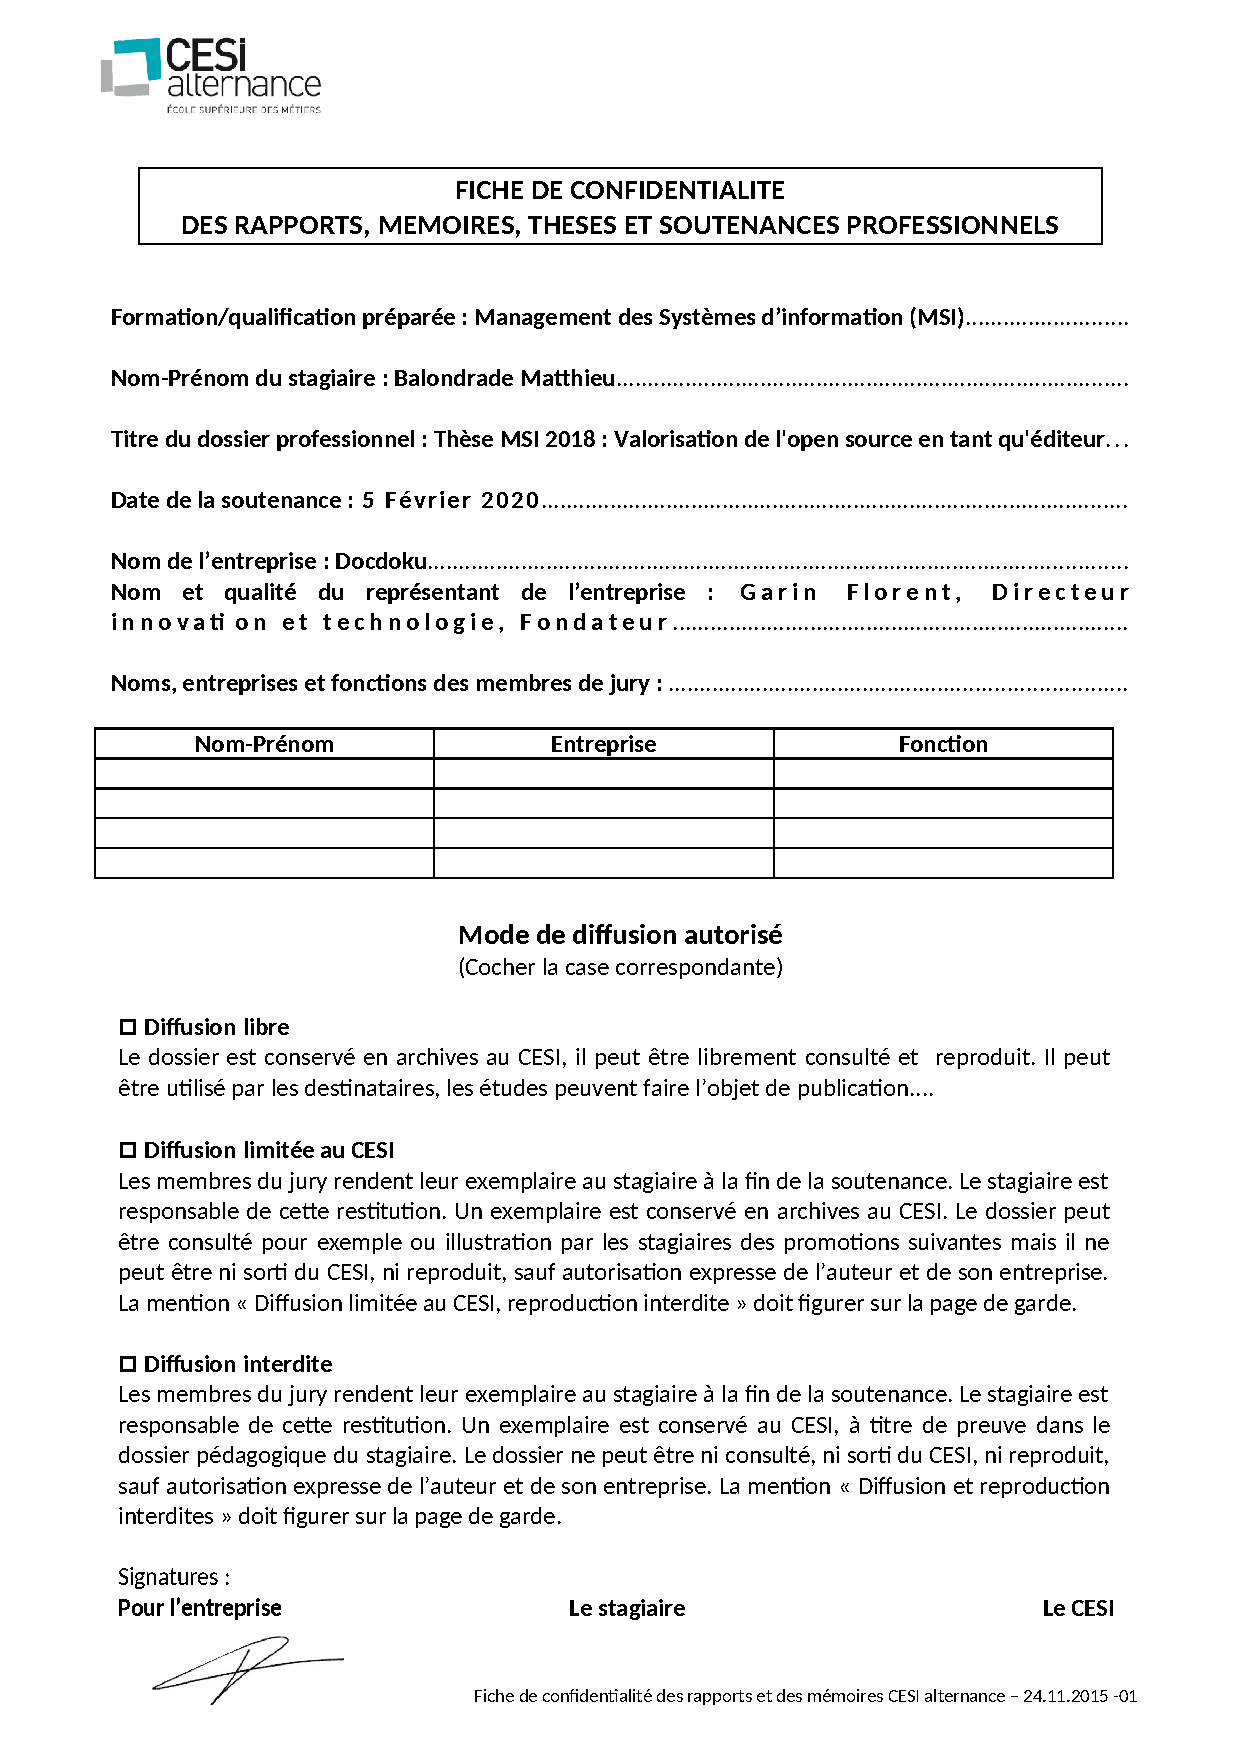
\includepdf[pages=-]{confidentialitecesi.pdf} % Fiche de confidentialité